% ----------------------------------------------------------------
% Report Class (This is a LaTeX2e document)  *********************
% ----------------------------------------------------------------
% Dissertation Template

\documentclass[11pt,oneside]{book}
% \usepackage[margin=1.2in]{geometry}
\usepackage[toc,page]{appendix}
\usepackage{graphicx}
%\usepackage{natbib}
\usepackage{lipsum}
\usepackage{caption}
\usepackage[numbers]{natbib}

%\documentclass[12pt,a4paper]{report}

\usepackage[lmargin=3.81cm,tmargin=2.54cm,rmargin=2.54cm,bmargin=2.52cm]{geometry}
\usepackage{mathptmx}

\begin{document}
\setcounter{tocdepth}{0} 
\renewcommand\labelitemi{---}

\frontmatter

\begin{titlepage}
\begin{center}
{\LARGE University of Sheffield}\\[1.5cm]
\linespread{1.2}\Large {\bfseries EEE339}\\[2cm]
\linespread{1}

\includegraphics[width=9cm]{images/logo.png}\\[1.5cm]

\linespread{1.2}\Large {\bfseries Digital Signal Processing Coursework}\\[1cm]
{\Large Mohammed Ayman Shaikh}\\[1cm]
\large A report submitted in fulfillment of the module\\EEE339 Digital Engineering\\[0.3cm] 
\textit{in the}\\[0.3cm]
School of Electronic and Electrical Engineering\\[2cm]
\today
\end{center}

\end{titlepage}


\linespread{1.5}

% Fonts -- the following two packages give you Times Roman in LaTex
%\usepackage{txfonts}


\pagenumbering{arabic}


\chapter{Introduction}
In this coursework, digital filters will be implemented in MATLAB to remove noise from 
\\Electrocardiogram (ECG) signals. ECG
\chapter{Main Body}
Below, two plots can be seen. The first plot
\begin{center}
%\centering
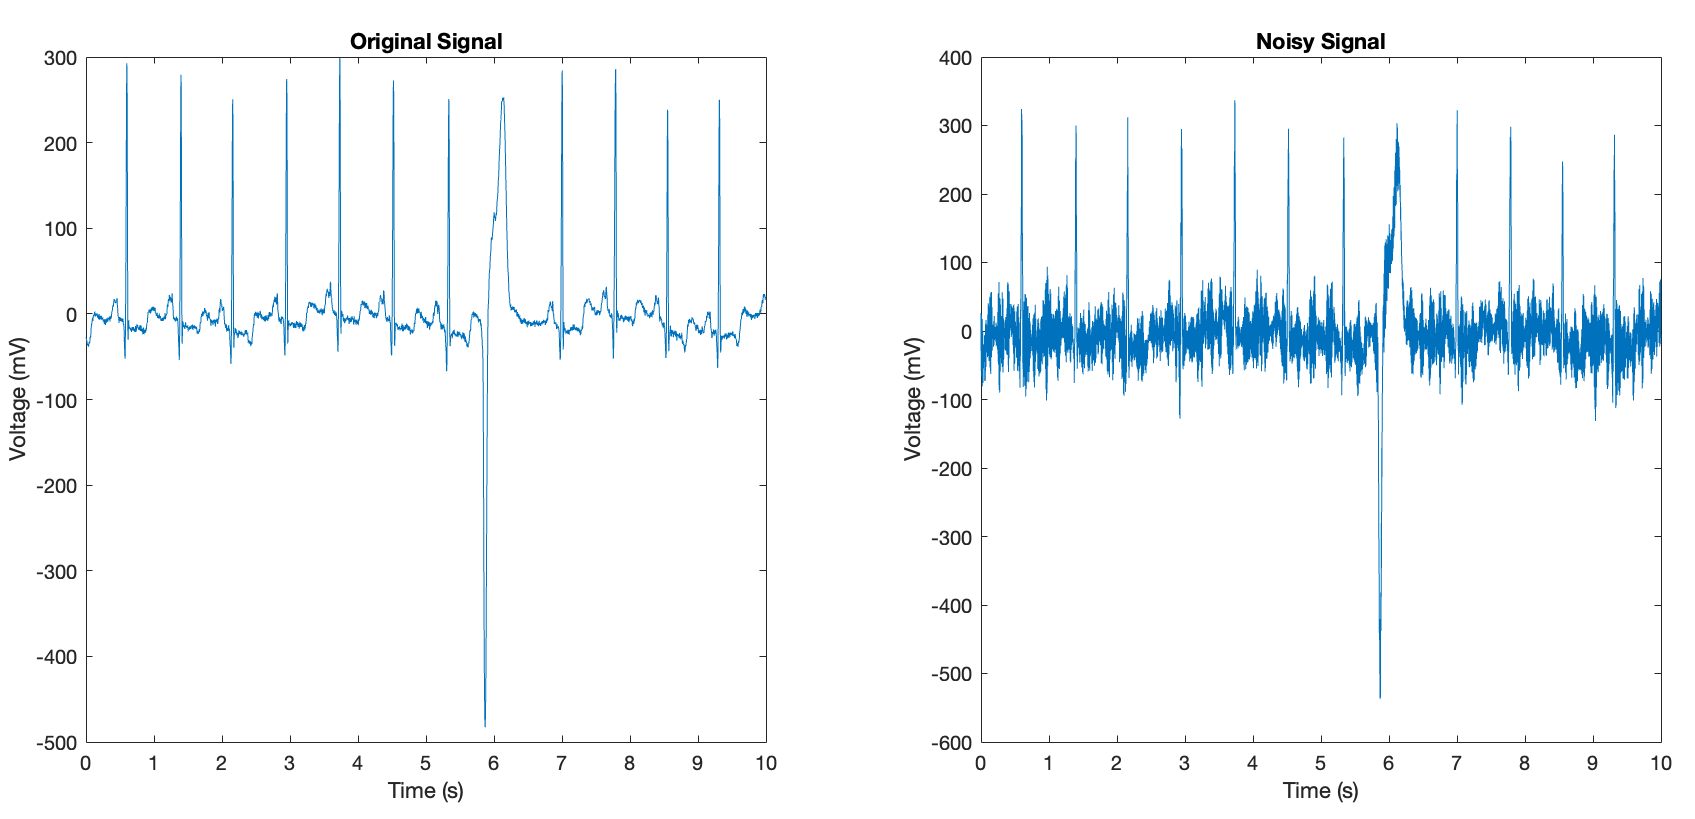
\includegraphics[width=18cm]{graphics/original_noisy_side_by_side.png}
\end{center}


\end{document}
% ----------------------------------------------------------------

